\documentclass{article}

\usepackage{polski}
\usepackage[utf8]{inputenc}
\usepackage{graphicx}
\usepackage{float}



\title{\Huge{
  \indexspace \textbf{Politechnika Poznańska Wydział Elektryczny}  \indexspace Telefonia IP \indexspace Komunikator głosowy VoIP \indexspace \textbf{"Pytler"}}}

\author{Patryk Mroczyński \\ \textit{patryk.mroczynski@student.put.poznan.pl} \\126810\\
        \\
        Daniel Staśczak \\ \textit{daniel.stasczak@student.put.poznan.pl} \\126816 \\}

\begin{document}

  \pagenumbering{gobble}
  \maketitle
  \newpage
  \tableofcontents
  \newpage
  \pagenumbering{arabic}

  \section{Charakterystyka ogólna projektu}
  \paragraph{} Pytler to komunikator działający w technologii VoIP. Umożliwia on wykonywanie połączeń głosowych między dwoma osobami. Aplikacja obsługuje funkcjonalności takie jak zarządzanie listą znajomych, na której użytkownik może zobaczyć status oraz opis tekstowy swoich znajomych, oraz ustawianie indywidualnych dzwonków dla każdego kontaktu.
  \section{Architektura systemu}
  \paragraph{} System oparty jest na modelu klient-serwer, w którym klient (łącznie z logiką po stronie klienta i interfejsem) jest uruchamiany na komputerze użytkownika jako aplikacja desktopowa, a na maszynie serwerowej działa silnik relacyjnej bazy danych oraz program ją obsługujący i wykonujący operacje takie jak obsługa komunikacji między aplikacjami klienckimi oraz zarządzanie kontami użytkowników.
  Serwer jedynie pośredniczy w nawiązywaniu połączenia, natomiast właściwa rozmowa przebiega bez jego uczestnictwa (klient-klient).
  \subsection{Mikroserwisy}
  W podrozdziale zostały wylistowane mikroserwisy wraz z dostępnymi dla nich metodami.
  \begin{itemize}
    \item UserApi
    \begin{itemize}
      \item GET /api/users- zwraca informacje o użytkowniku.
      \item PUT /api/users/:token - umożliwia użytkownikowi na zmianę ustawień.
      \item DELETE /api/users/:id - usuwa konto użytkownika.
    \end{itemize}

    \item AuthApi
    \begin{itemize}
      \item GET /api/auth- zwraca token uwierzytelniający.
      \item POST /api/auth - tworzy nowego użytkownika.
      \item PATCH /api/auth/:token - aktywuje konto użytkownika.
    \end{itemize}

    \item ContactApi
    \begin{itemize}
      \item GET /api/contacts/:id - zwraca listę kontaktów dla użytkownika.
      \item POST /api/contacts/ - dodaje zaproszenie do znajomych.
      \item DELETE /api/contacts/:id - usuwa kontakt z listy znajomych.
    \end{itemize}

    \item InvitationApi
    \begin{itemize}
      \item GET /api/invitations - zwraca listę zaproszeń do użytkownika.
      \item PUT /api/invitations - aktualizuje stan zaproszenia.
    \end{itemize}

    \item SessionsApi
    \begin{itemize}
      \item GET /api/sessions/:id - zwraca informację o tym, czy użytkownik ma aktualną sesję.
      \item PUT /api/sessions - przedłuża lub kończy sesję.
      \item POST /api/sessions/:id - tworzy nową sesję.
    \end{itemize}

    \item CallSessionsApi
    \begin{itemize}
      \item GET /api/callsessions/:id - zwraca informację o tym, czy użytkownik ma aktualną sesję rozmowy.
      \item PUT /api/callsessions - przedłuża lub kończy sesję rozmowy.
      \item POST /api/callsessions/:id - tworzy nową sesję rozmowy.
    \end{itemize}

    \item PendingCallsApi
    \begin{itemize}
      \item GET /api/pendingcalls - pobiera informacje o oczekujących połączeniach.
      \item POST /api/pendingcalls - tworzy nowe informacje o oczekującym połączeniu.
      \item DELETE /api/pendingcalls - usuwa wpis o oczekującym połączeniu.
    \end{itemize}


  \end{itemize}
  \section{Wymagania}
  \paragraph{} W rozdziale opisane są wymagania funkcjonalne oraz niefunkcjonalne z podziałem na aktorów.
  \subsection{Wymagania funkcjonalne}
  \begin{enumerate}
    \item Niezalogowany użytkownik może się zarejestrować.
    \item Niezalogowany użytkownik może się zalogować.
    \item Zalogowany użytkownik może wysłać innemu zarejestrowanemu użytkownikowi zaproszenie do swojej listy znajomych.
    \item Zaproszenie do znajomych może zostać zaakceptowane lub odrzucone.
    \item Zalogowany użytkownik może usunąć znajomego z listy znajomych.
    \item Zalogowany użytkownik może zadzwonić do użytkownika ze swojej listy znajomych.
    \item Użytkownik, do którego jest wykonywane połączenie może je odrzucić lub odebrać.
    % \item Podczas rozmowy możliwe jest wyciszenie mikrofonu i dźwięku za pośrednictwem interfejsu aplikacji.
    % \item Użytkownik ma możliwość ustawienia indywidualnego utworu dźwiękowego dla próby połączenia od każdego z listy znajomych.
    \item Zalogowany użytkownik ma możliwość ustawienia opisu i zdjęcia profilowego, które będą wyświetlane jego znajomym.
    \item Użytkownik inicjujący rozmowę może wybrać między połączeniem nieszyfrowanym a szyfrowanym.
    \item Zalogowany użytkownik może zmienić swoje hasło oraz adres e-mail.
  \end{enumerate}
  \subsection{Wymagania niefunkcjonalne}
  \begin{enumerate}
    \item Aby użytkownik mógł korzystać z funkcjonalności serwisu musi być zalogowany.
    \item Dane użytkownika są przechowywane w bazie danych.
    \item Hasło użytkownika jest przechowywane jako wynik funkcji skrótu SHA-256.
    \item Aplikacja działa w architekturze klient-serwer.
    \item Aplikacja serwerowa wykorzystuje relacyjną bazę danych.
    %\item Podczas oczekiwania na rozmowę użytkownikowi odtwarza się utwór Jana Sebastiana Bacha - “Bouree In E Minor”.
    %\item Po odebraniu połączenia użytkownikowi zostaje odtworzony krótki sygnał dźwiękowy.
    \item Próba wykonania połączenia do użytkownika, który aktualnie rozmawia lub nie jest zalogowany kończy się niepowodzeniem.
    \item Użytkownik, do którego próba połączenia się nie powiodła otrzymuje informację tekstową.
    \item Użytkownik podczas próby połączenia do niego słyszy utwór dźwiękowy.
    \item Połączenia szyfrowane używają szyfrowania symetrycznego AES-256 z wymianą kluczy poprzez algorytm Diffiego-Hellmana.
    \item Oczekiwanie na odebranie połączenia trwa maksymalnie 15 sekund, po czym automatycznie zostaje ono odrzucone.
    \item Do korzystania z aplikacji wymagane jest posiadanie mikrofonu oraz słuchawek lub głośników.
    \item W trakcie komunikacji między aplikacją kliencką a serwerową używany jest protokół TCP.
    \item W trakcie rozmowy między użytkownikami wykorzystywany jest protokół UDP.
    \item Do kompresji dźwięku podczas rozmowy między użytkownikami wykorzystywany jest kodek ADPCM.
    \item Logowanie wymaga podania przez użytkownika loginu (nazwa użytkownika) oraz hasła.
    % \item Zdjęcia profilowe oraz wybrane przez użytkownika dzwonki przechowywane są na serwerze.
    \item Zdjęcia profilowe przechowywane są na serwerze.
    \item Autoryzowanie użytkownika odbywa się za pomocą metody Basic Auth.
    \item Hasło użytkownika musi mieć co najmniej 8 znaków, w tym co najmniej jedną cyfrę, jedną wielką literę i jedną małą literę
  \end{enumerate}
  \section{Narzędzia}
  \paragraph{}Serwer działa w oparciu o system operacyjny Ubuntu Server 18.04 LTS. Zarządzanie danymi jest oparte na relacyjnej bazie danych PostgreSQL. Aplikacja kliencka jest wspierana na wybranych systemach operacyjnych z rodziny Windows oraz na systemie operacyjnym Linux. Wybrane języki programowania to Python 3.6, zarówno dla aplikacji serwerowej, jak i aplikacji klienckiej. Główne moduły tego języka, zastosowane w systemie, to CherryPy (do implementacji REST API, na którym opiera się sposób działania aplikacji serwerowej), PyAudio (do implementacji nagrywania oraz odtwarzania dźwięku w aplikacji klienckiej) oraz Tkinter (do implementacji GUI w aplikacji klienckiej).
  Pracę zespołową wspierają:
  \begin{enumerate}
    \item System kontroli wersji Git, hostowany w serwisie GitHub.
    \item Latex w dystrybucji Texlive.
    \item Narzędzie do zarządzania bazami danych DBeaver.
    \item Komunikator głosowy Discord.
  \end{enumerate}
  \section{Schemat bazy danych}
  \paragraph{} W rozdziale opisane zostały wykorzystane tabele oraz relacje zachodzące pomiędzy nimi.
    \begin{figure}[H]
      \centering
        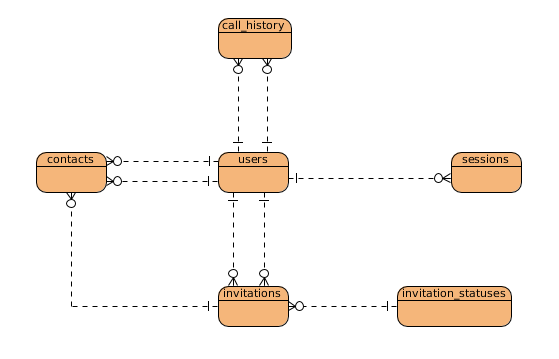
\includegraphics[width=1.0\linewidth]{assets/erd.png}
        \caption[]{Diagram związków encji}
        \label{fig:er}
    \end{figure}

    Zgodnie z rysunkiem \ref{fig:er}, w bazie danych znajduje się dziesięć tabel. Tabela \texttt{users} zawiera informacje o zarejestrowanych użytkownikach - m.in. ich nazwę konta, hasło przechowywane jako wynik funkcji skrótu oraz adres email. Odwołania do tej tabeli znajdują się w tabelach \texttt{sessions}, która przechowuje informacje o sesjach - o ich czasie rozpoczęcia oraz zakończenia, \texttt{invitations}, która zawiera informacje o zaproszeniach do listy znajomych wysyłanych przez użytkowników, \texttt{contacts}, w której znajdują się wpisy o kontaktach poszczególnych użytkowników, \texttt{keys}, przyporządkowującej rózne rodzaje kluczy do danego użytkownika oraz w tabeli \texttt{call\_history}, która przechowuje dane o historiach połączeń pomiędzy użytkownikami. Dostępne statusy zaproszeń znajdują się w tabeli \texttt{invitation\_statuses}, natomiast dostępne rodzaje kluczy (np. służący aktywacji konta lub zmianie hasła) znaleźć można w tabeli \texttt{key\_types}. Dodatkowo istnieją dwie tabele wspomagające połączenia pomiędzy użytkownikami - \texttt{call\_sessions}, w której są zapisane informacje o sesjach połączeń głosowych oraz \texttt{pending\_calls}, która pośredniczy w wymianie ustawień połączenia między użytkownikami.

    \begin{figure}[H]
      \centering
        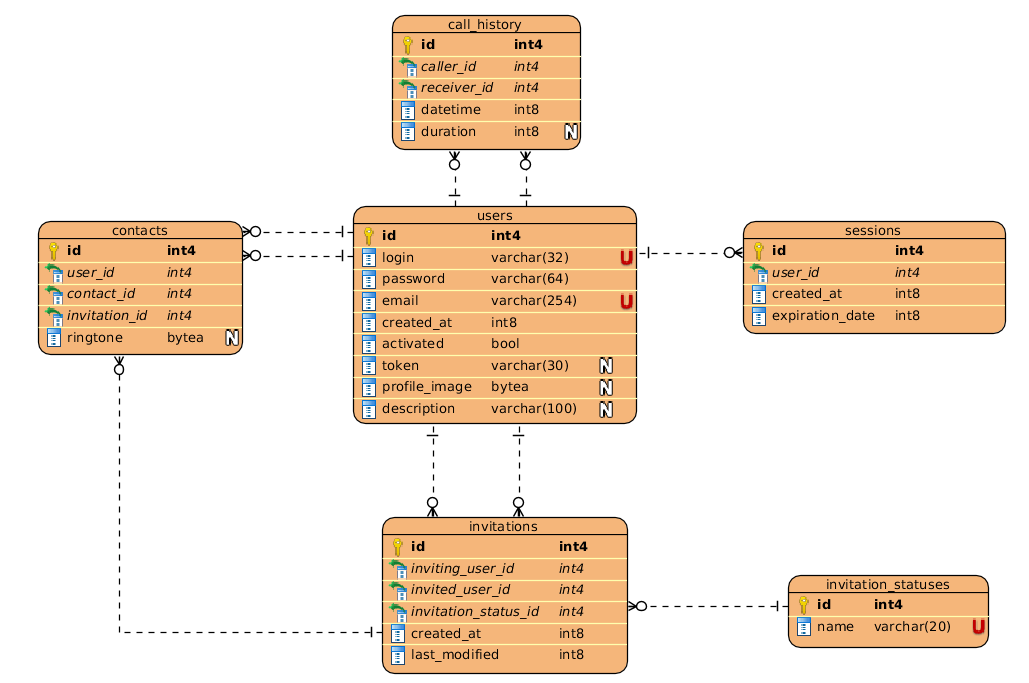
\includegraphics[width=1.0\linewidth]{assets/rel.png}
        \caption[]{Model relacyjny}
        \label{fig:rel}
    \end{figure}

    Na rysunku \ref{fig:rel} znajduje się rozwinięcie diagramu związków encji do modelu relacyjnego. Prezentuje on kolumny, które należą do poszczególnych tabel wraz z oznaczeniem kluczy głównych (żółty klucz) i obcych (zielona strzałka). Opcjonalność wartości w kolumnach jest oznaczona białą literą "N", a unikalność czerwoną literą "U".

    \section{Diagramy UML}
    \paragraph{} W rozdziale znajdują się diagramy UML wraz z ich opisami.

    \subsection{Diagramy przypadków użycia}
    W rozdziale zostały opisane diagramy przypadków użycia dla użytkownika zalogowanego i niezalogowanego.

    \begin{figure}[H]
      \centering
        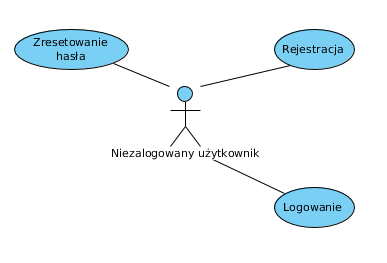
\includegraphics[width=1.0\linewidth]{assets/dpu1.png}
        \caption[]{Diagram przypadków użycia dla użytkownika niezalogowanego}
        \label{fig:dpu1}
    \end{figure}

    Zgodnie z rysunkiem \ref{fig:dpu1}, użytkownik niezalogowany może wykonać trzy operacje - logowanie, rejestrację oraz resetowanie hasła.

    \begin{figure}[H]
      \centering
        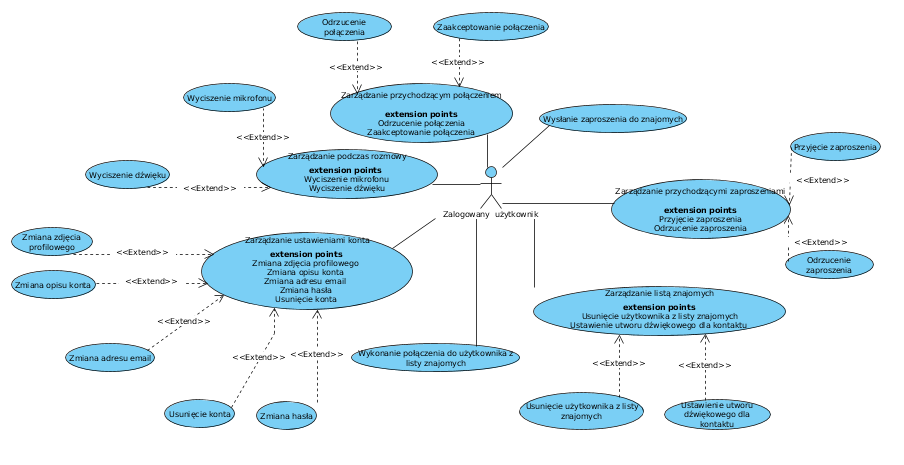
\includegraphics[width=1.0\linewidth]{assets/dpu2.png}
        \caption[]{Diagram przypadków użycia dla użytkownika zalogowanego}
        \label{fig:dpu2}
    \end{figure}

    Rysunek \ref{fig:dpu2} przedstawia możliwe czynności, które może wykonać użytkownik zalogowany. Najważniejsze czynności to m.in. zarządzanie listą znajomych, zarządzanie ustawieniami konta oraz działania związane z inicjowaniem oraz prowadzeniem rozmowy.
\end{document}
